\section{Elektronrör}
\label{elektronrör}
\index{elektronrör}

\subsection{Allmänt}

Ett elektronrör består av två eller flera elektroder i en lufttom glaskolv.

\subsection{Vakuumdioden (tvåelektrodröret)}
\textbf{HAREC a.\ref{HAREC.a.2.8.1}\label{myHAREC.a.2.8.1}}
\label{vakuumdioden}
\index{vakuumdioden}
\index{elektronrör!diod}
\index{anod}
\index{katod}

\begin{wrapfigure}[9]{R}{0.5\textwidth}
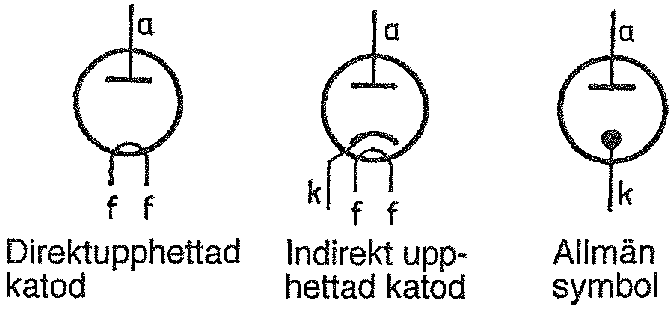
\includegraphics[width=0.5\textwidth]{images/cropped_pdfs/bild_2_2-24.pdf}
\caption{Schemasymboler för dioder}
\label{fig:BildII2-24}
\end{wrapfigure}

Bild \ref{fig:BildII2-24}

Dioden innehåller två elektroder anod (a) och katod (k), med f där
f = glödtråd (filament).

\emph{Anoden} ska dra elektronerna från katoden.
\emph{Katoden} ska avge elektronerna och måste därför hettas upp.

Upphettningen av katoden görs antingen med direkt upphettning, det vill säga katoden
är i sig själv en glödtråd, där en 4- till 6-volts strömkälla är vanligt, eller
med indirekt upphettning, det vill säga en glödtråd omsluter och hettar upp ett
speciellt katodmaterial, där en 1,5 till 12,6~volts glödströmkälla är vanligt.

\subsubsection{Edisoneffekten}
\index{Edisoneffekten}
\index{elektronrör!Edisoneffekten}

\begin{wrapfigure}[12]{R}{0.5\textwidth}
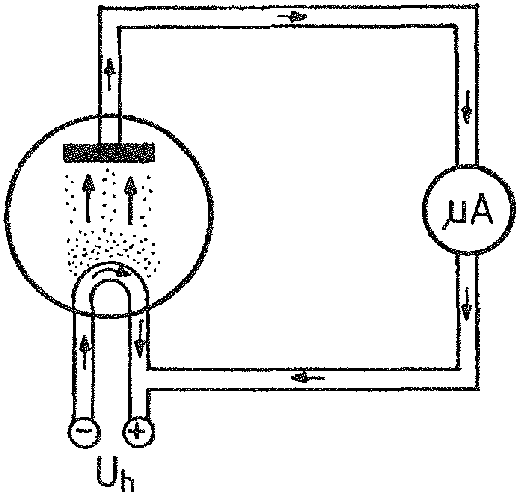
\includegraphics[width=0.5\textwidth]{images/cropped_pdfs/bild_2_2-25.pdf}
\caption{Edisoneffekten}
\label{fig:BildII2-25}
\end{wrapfigure}

Bild \ref{fig:BildII2-25} illustrerar \emph{Edisoneffekten}, det vill säga när katoden
upphettas lossnar fria elektroner från den och bildar ett moln.
Med en spänning mellan anod och katod, med anoden positiv, så kommer
elektronerna att dras mot anoden.
En s.k. anodström börjar att flyta.

\subsubsection{\(I_a/U_a\)-karaktäristikan för en vakuumdiod}

\begin{figure}
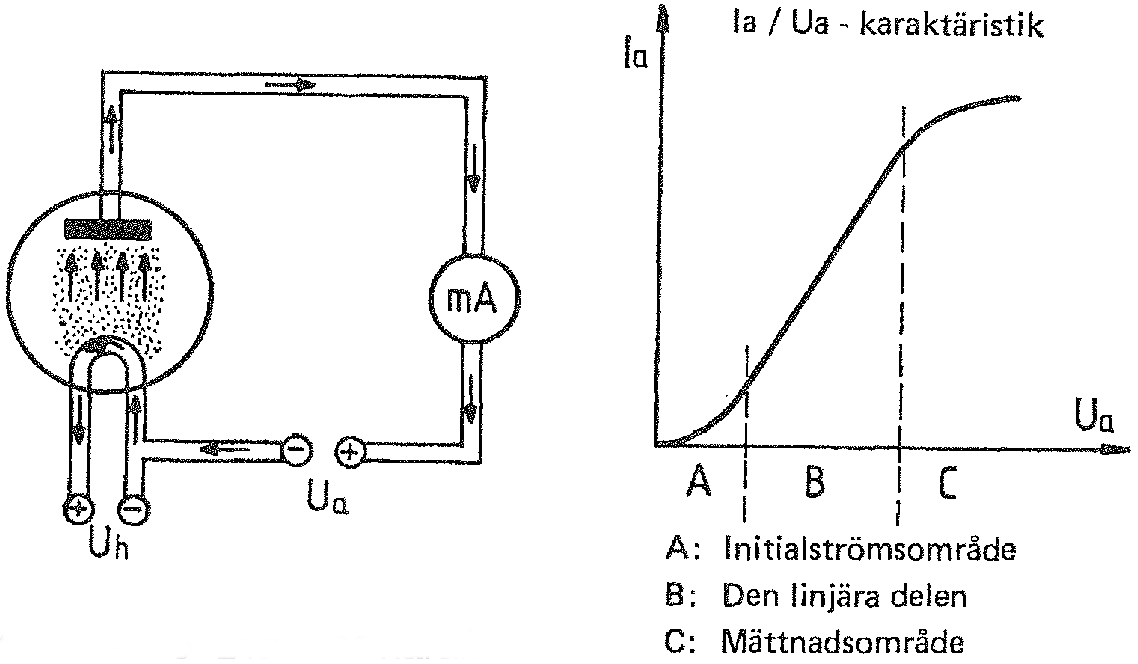
\includegraphics[width=\textwidth]{images/cropped_pdfs/bild_2_2-26.pdf}
\caption{Diodens karaktäristik}
\label{fig:BildII2-26}
\end{figure}

Bild \ref{fig:BildII2-26} illustrerar rördiodesn karakteristik.
När anoden ges positiv potential (anodspänning), flyter en elektronström från
katod till anod (anodström).
Om anodspänningen \(U_a\) ökar så ökar anodströmmen \(I_a\).
Varje par av talvärden representerar en punkt i ett diagram, som det på bilden.
När anodspänningen ökat till ett visst värde, så ökar inte anodströmmen
ytterligare.
I ett mellanområde är kurvan i det närmaste rak.

\subsubsection{Likriktarverkan}
\index{elektronrör!likriktarverkan}

När anoden i en vakuumdiod ges positiv potential i förhållande till katoden,
flyter en s.k. anodström förutsatt att katoden upphettas så att den avger fria
elektroner.

När anoden ges en negativ potential i förhållande till katoden flyter däremot
ingen anodström.

Vakuumdioden kan därför användas för likriktning av växelströmmar. Den har en
likriktande funktion.

\subsubsection{Halvvågslikriktning}

\begin{figure}
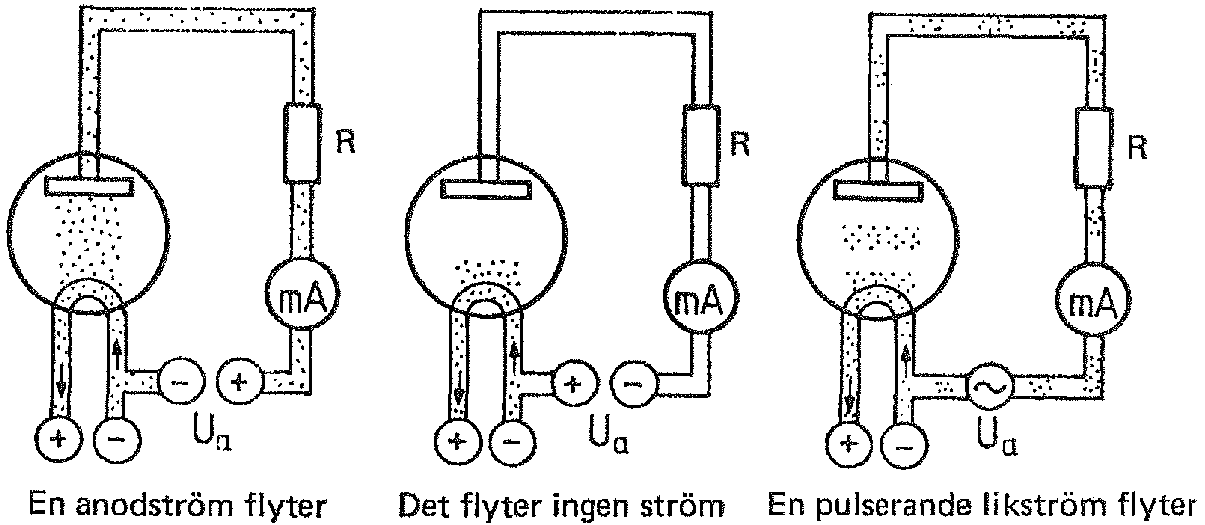
\includegraphics[width=\textwidth]{images/cropped_pdfs/bild_2_2-27.pdf}
\caption{Halvvågslikriktning}
\label{fig:BildII2-27}
\end{figure}

Bild \ref{fig:BildII2-27} illustrerar halvvågslikriktning.
När anoden ges en omväxlande positiv och negativ potential, en växelspänning, så
flyter anodström under varje positiv halvperiod av växelspänningen.
En likströmspuls uppstår under varannan halvperiod.

\subsubsection{Helvågslikriktning}

\begin{figure}
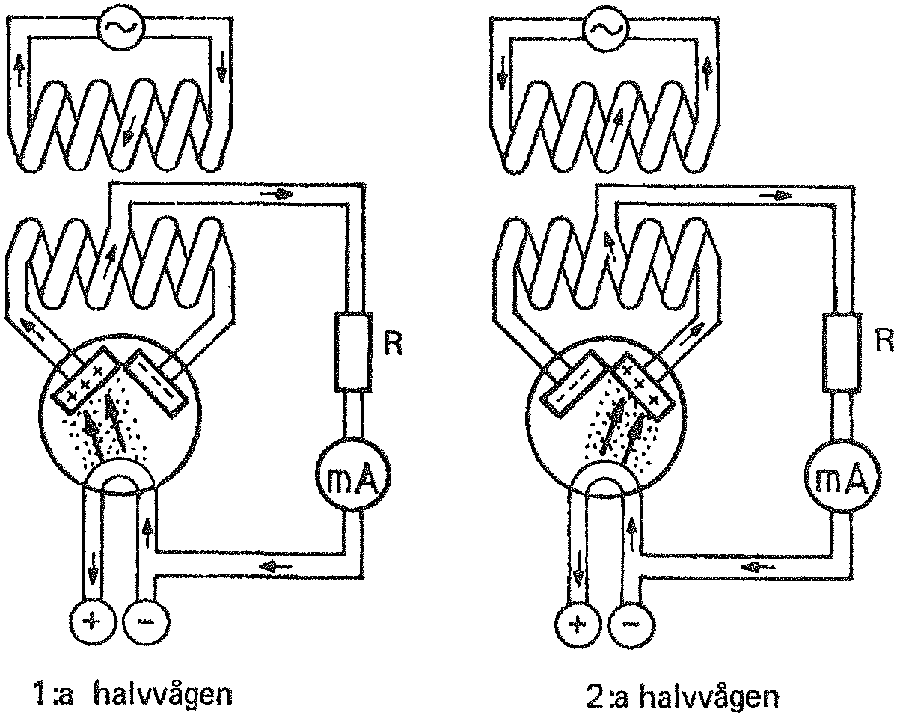
\includegraphics[width=\textwidth]{images/cropped_pdfs/bild_2_2-28.pdf}
\caption{Helvågslikriktning}
\label{fig:BildII2-28}
\end{figure}

Bild \ref{fig:BildII2-28} illustrerar halvvågslikriktning.
Med ett elektronrör med dubbla anoder och en transformator med mittuttag på
sekundärlindningen, kan växelspänningens båda halvperioder utnyttjas så, att
anodström flyter i samma riktning under alla halvperioder.

\begin{figure}
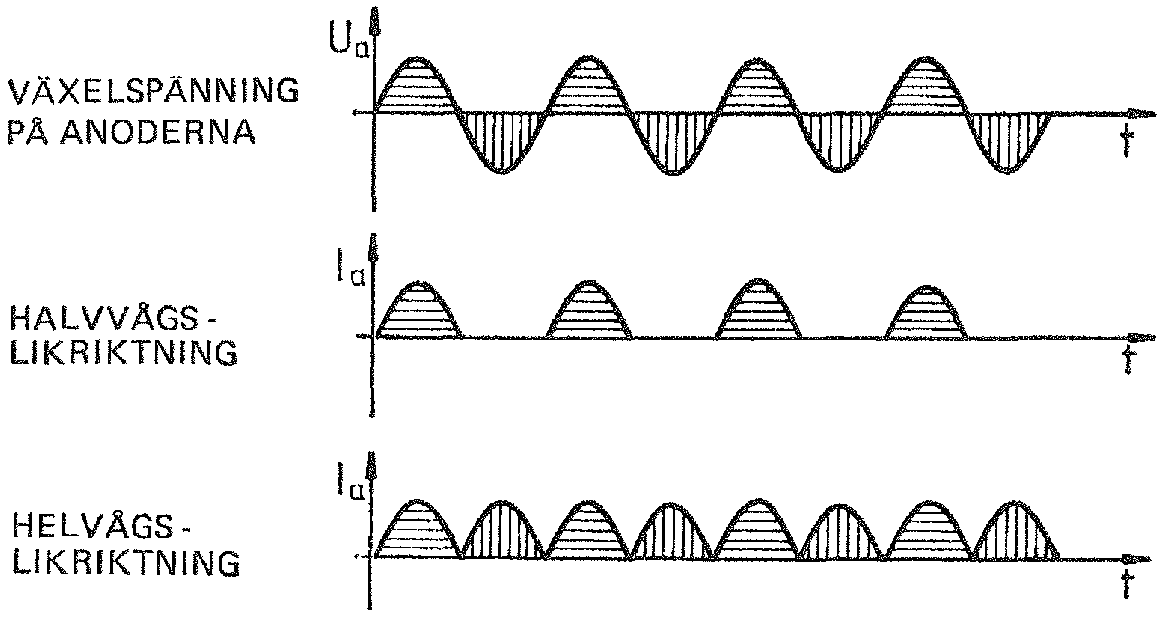
\includegraphics[width=\textwidth]{images/cropped_pdfs/bild_2_2-29.pdf}
\caption{Likriktande funktion}
\label{fig:BildII2-29}
\end{figure}

Bild \ref{fig:BildII2-29} illustrerar hur växelspännng via två
två halvvågslikriktningar formar en helvågslikriktning.

\subsection{Vakuumtrioden (treelektrodröret)}
\index{vakuumtrioden}
\index{trioden}
\index{elektronrör!triod}

\begin{figure*}[ht]
\begin{center}
  %%\begin{wrapfigure}[9]{R}{0.5\textwidth}
  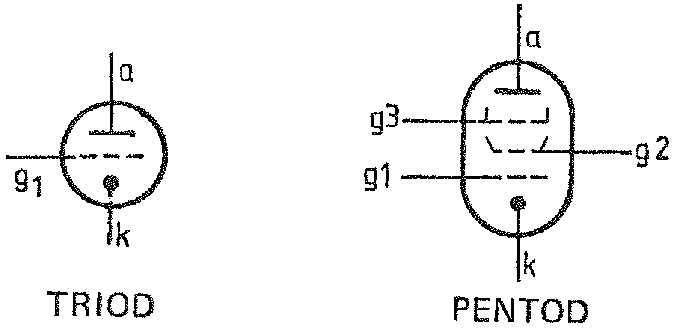
\includegraphics[width=0.5\textwidth]{images/cropped_pdfs/bild_2_2-30.pdf}
  \caption{Symboler för triod och pentod}
  \label{fig:BildII2-30}
  %%\end{wrapfigure}
\end{center}
\end{figure*}

Bild \ref{fig:BildII2-30} illustrerar symboler för triod och pentod.

Trioden innehåller tre elektroder anod (a), styrgaller (\(g_1\)) och katod (k)
med glödtråd (f = filament).

\subsubsection{Triodens funktion}

Bild \ref{fig:BildII2-31} illustrerar en triod och dess elektronström.
En triod fungerar som en diod, när styrgallret ges samma potential som katoden.
Valet av förspänning avgör triodens arbetssätt.
Styrgallret kan ges positiv, neutral eller negativ potential (förspänning) i
förhållande till katoden.
Med styrgallret positivt ökar anodströmmen.
Med gallret negativt minskar den.

Trioden har en \emph{förstärkande} funktion eftersom anodströmmen kan styras med
styrgallret. En liten ändring av gallerspänningen medför stor ändring av
anodströmmen.
Vid positiv förspänning flyter det gallerström, som inte får bli för hög.
Vanligen väljs en negativ förspänning.

\begin{figure}[ht]
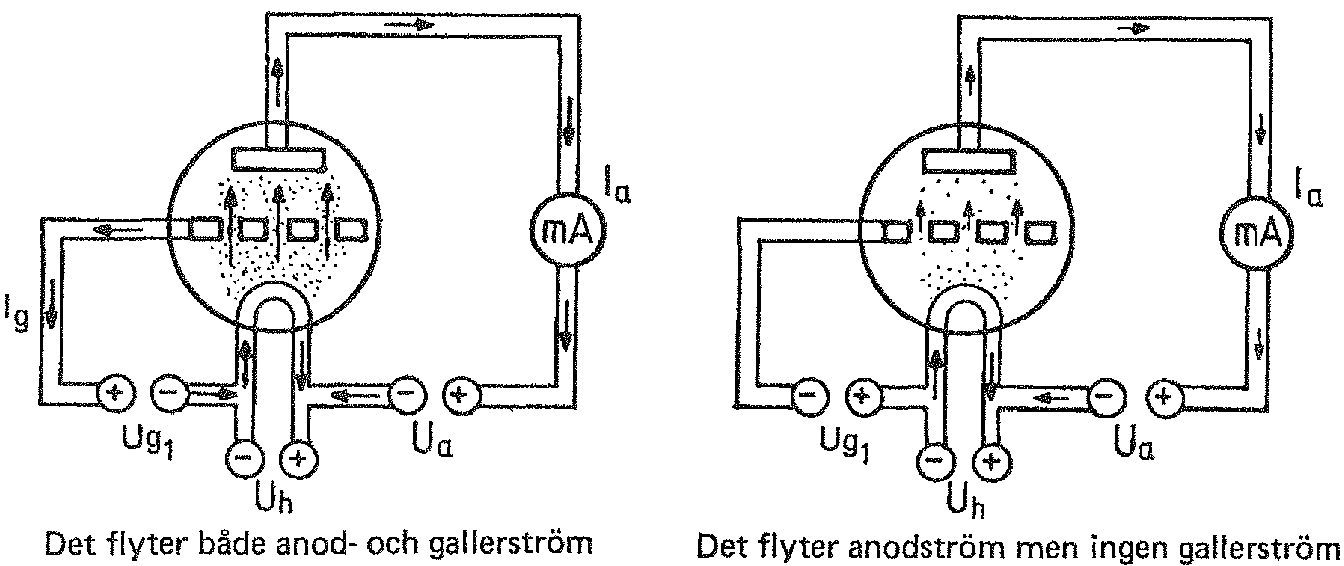
\includegraphics[width=\textwidth]{images/cropped_pdfs/bild_2_2-31.pdf}
\caption{Elektronstömmen i en triod}
\label{fig:BildII2-31}
\end{figure}

\subsubsection{Triodens strömkretsar och strömkällor}

\begin{tabular}{lll}
Glödströmskrets      & Anodkrets        &  Gallerkrets \\
Glödbatteri          & Anodbatteri      &  Gallerbatteri \\
Glödspänning \(U_f\) & Anodsp. \(U_a\)  &  Gallersp. \(U_{g1}\) \\
Glödström \(I_f\)    & Anodstr. \(I_a\) &  Gallerstr. \(I_{g1}\) \\
\end{tabular}

Vanligen används nätdrivna strömkällor i stället för batterier.

Valet av gallerförspänning är avgörande för triodens arbetssätt.

\subsection{Pentoden (femelektrodröret)}
\index{pentod}
\index{elektronrör!pentod}

Pentaden innehåller fem elektroder.

\begin{tabular}{ll}
  a       & anod \\
  \(g_3\) & bromsgaller \\
  \(g_2\) & skärmgaller \\
  \(g_1\) & styrgaller \\
  k      & katod, med f f = glödtråd (filament) \\
\end{tabular}

Bromsgallret förbinds med katoden. Skärmgallret ges en potential som är något
lägre än anodspänningen. Broms- och skärmgallren förhindrar elektronerna att
studsa tillbaka till styrgallret efter anslaget mot anoden.


\subsection{Tetroden (fyraelektrodröret)}
\index{tetrod}
\index{elektronrör!tetrod}

Denna rörtyp innehåller fyra elektroder. Uppbyggnaden är densamma som pentodens,
men bromsgallret saknas.

\subsection{Karaktäristika för elektronrör}

\begin{figure}
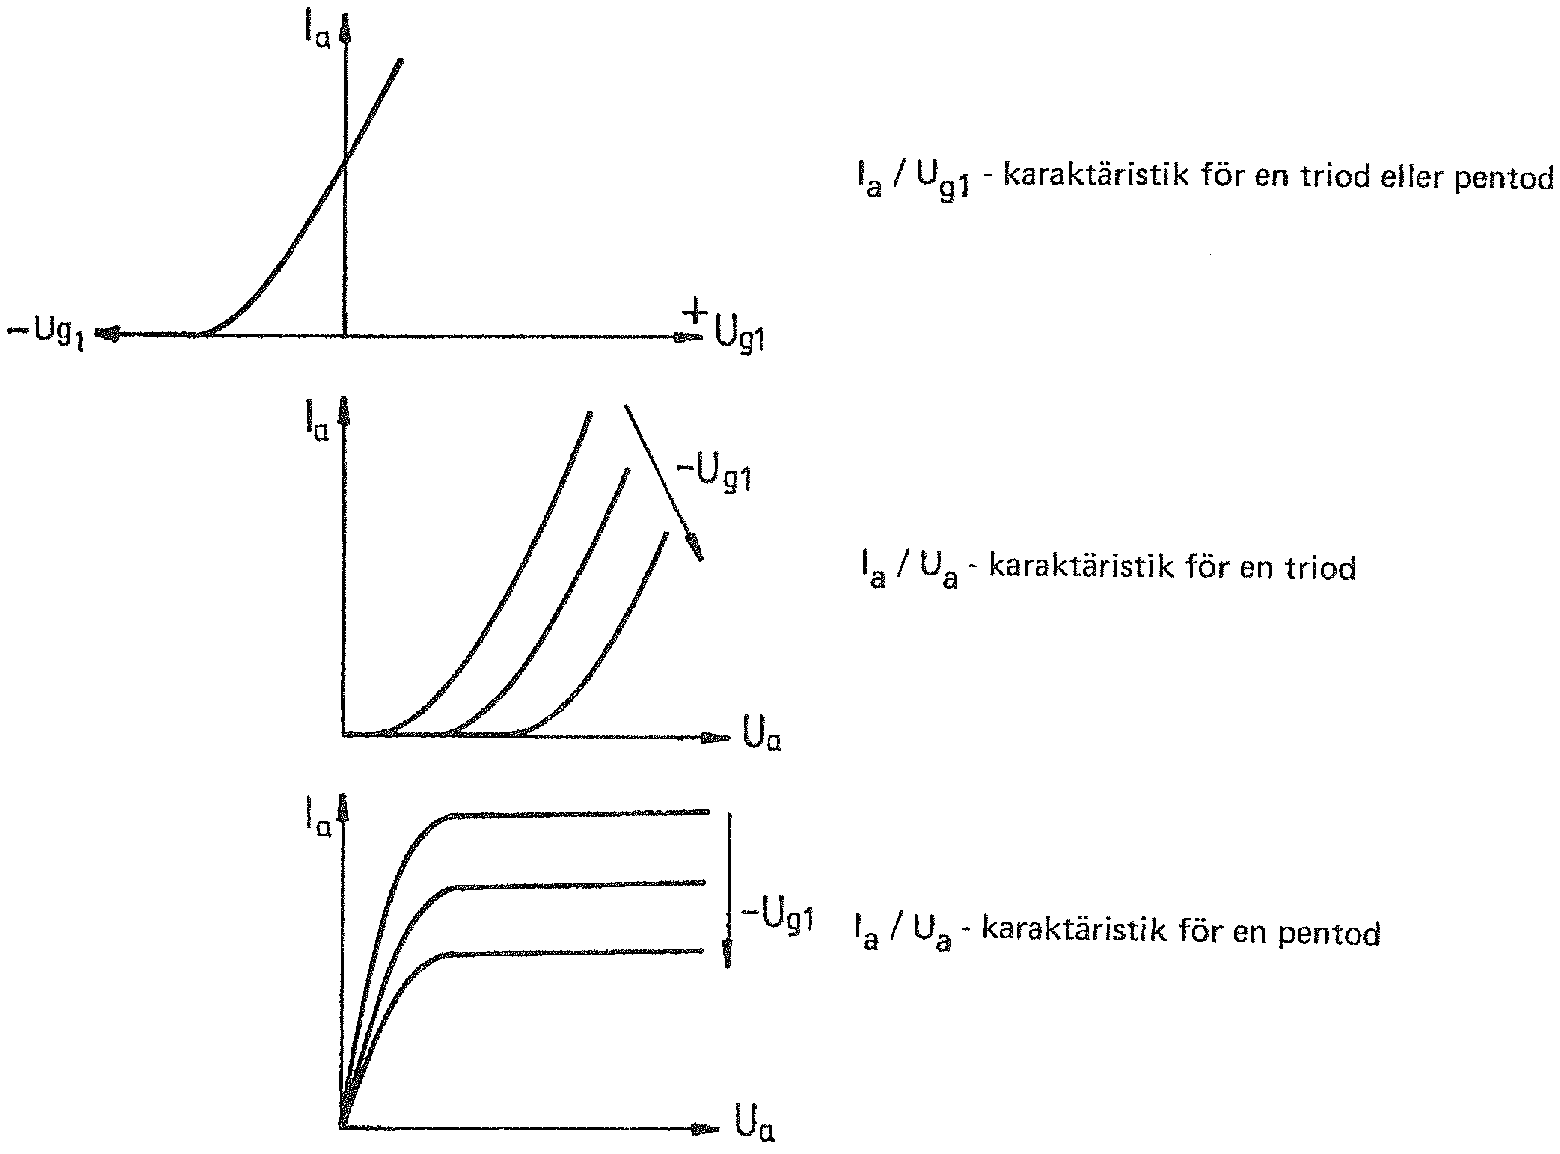
\includegraphics[width=\textwidth]{images/cropped_pdfs/bild_2_2-32.pdf}
\caption{Karaktäristika för elektronrör}
\label{fig:BildII2-32}
\end{figure}

Bild \ref{fig:BildII2-32} illustrerar ett \(I_a/U_{gt}\)-diagram för en triod
eller pentod, vid \(U_a\) = konstant

\begin{wrapfigure}[20]{R}{0.5\textwidth}
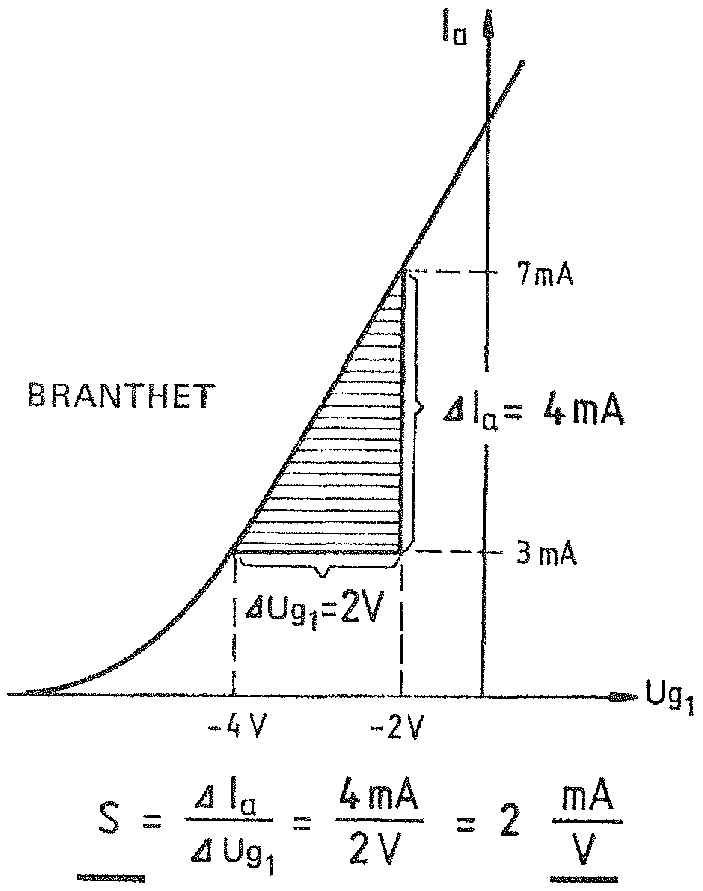
\includegraphics[width=0.5\textwidth]{images/cropped_pdfs/bild_2_2-33.pdf}
\caption{Branthet}
\label{fig:BildII2-33}
\end{wrapfigure}

\(I_a/U_a\)-diagram för en triod, vid \(U_{g1}\) = konstant

\(I_a/U_a\)-diagram för en pentod, vid \(U_{g1}\) = konstant

Tre kurvor visas i \(I_a/U_a\)-diagrammen, med olika värden på
\(U_{g1}\) = konstant (\(U_{g1}\) är s.k. parameter).

\subsection{Branthet $S$ och inre resistans $R_i$}

Bild \ref{fig:BildII2-33} visar brantheten.
Om man (vid konstant anodspänning) ändrar gallerförspänningen med värdet
\(\Delta U_{g1}\) så ändrar sig anodströmmen med värdet \(\Delta I_a\).

Branthet \(S = \dfrac{\Delta I_a}{\Delta U_{g1}}\)

\(S\ [mA/V]\) \(\Delta I_a\ [mA]\) \(U_{g1}\ [V]\)

Bild \ref{fig:BildII2-34} visar den inre resistansen.
Om man (vid konstant gallerförspänning) ändrar anodspänningen med
\(\Delta U_a\) så ändras anodströmmen med värdet \(\Delta I_a\).

Inre resistans \(R_i = \dfrac{\Delta U_a}{\Delta I_a}\)

\(R_i\ [k \omega]\)  \(\Delta U_a\ [V]\)  \(\Delta I_a\ [mA]\)

\begin{figure}[ht]
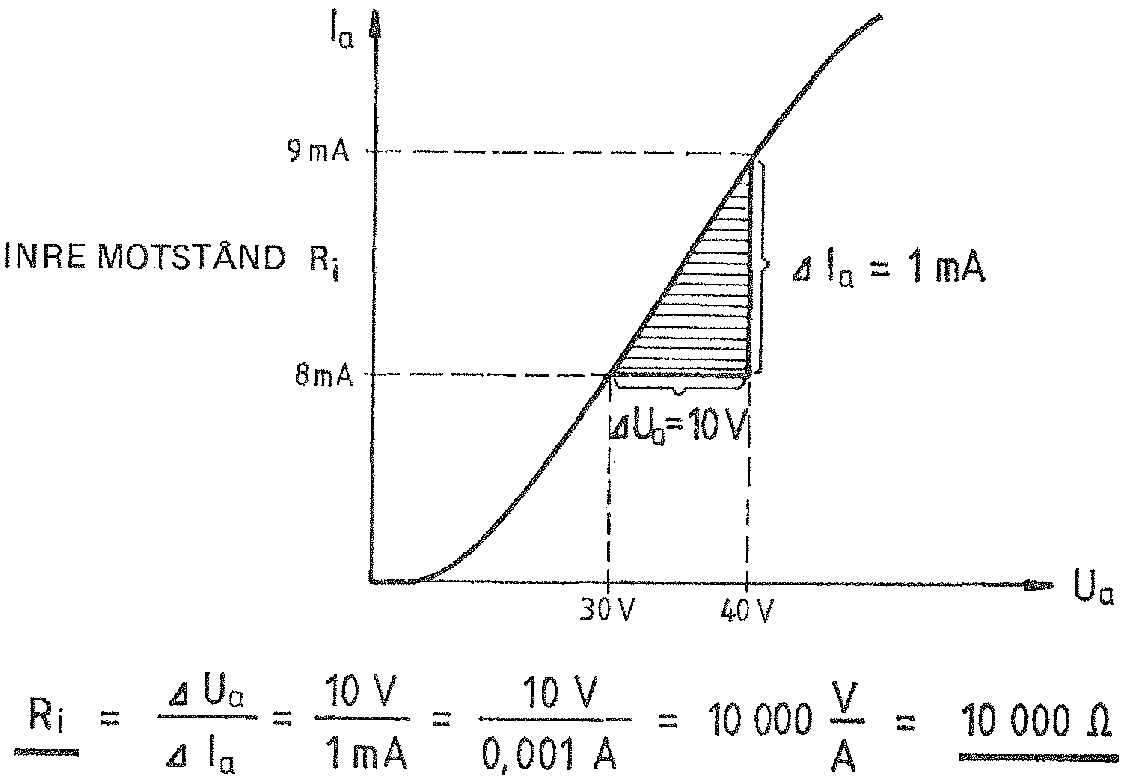
\includegraphics[width=\textwidth]{images/cropped_pdfs/bild_2_2-34.pdf}
\caption{Inre resistans}
\label{fig:BildII2-34}
\end{figure}

Om man vill ändra anodströmmen med \(\Delta I_a\), så ges det två möjligheter,
antingen ändra gallerförspänningen med värdet \(\Delta U_{g1}\)
eller ändra anodspänningen med värdet \(\Delta U_a\).
Med ändring av gallerförspänningen med värdet \(U_{g1}\) kan man åstadkomma
samma anodströmsändring \(\Delta I_a\) som med en ändring av anodspänningen
med värdet \(\Delta U_a\).

\subsection{Barkhausens elektronrörsformler}
\index{Barkhausen elektronrörsformler}
\index{elektronrör!Barkhausen formler}

Förstärkningsfaktorn \(\mu \) illustreras av följande samband gäller mellan de s.k. rörkonstanterna

\(\mu = S \cdot R_i\)

\emph{Exempel:}
Beräkna \(\mu\)  om \(S = 2\ mA/V\) \(R = 10\ k\Omega\) \(\mu = ?\)

\emph{Svar:} \(\mu = 20\) (\(\mu\)  är dimensionslös)

\subsection{Transistorer jämfört med elektronrör}

Transistorer har fördelar som lågt pris, små dimensioner, lång livslängd,
enkel strömförsörjning (glödström behövs inte) and låg driftspänning (6~V,
12~V \ldots ). Nackdelen som traditionellt finns är känslighet för
överbelastning och höga temperaturer.

Elektronrör har fördelen av tålighet mot överbelastning, men bland nackdelarna
har man att man behöver hög anodspänning, behöver glödström samt att de är
utrymmeskrävande.

Ett användningsområde, där elektronrör ännu är vanliga, är i större
sändarslutsteg.

Transistorer ersätter numera nästan helt elektronrören, men man bör ändå känna
elektronrörens egenskaper och arbetssätt.
